% siminos/blog/Lyapunov.tex
% $Author$ $Date$

\chapter{Lyapunov vectors}
\label{s:LyapunovVec}

This part of the blog focuses on the use of `covariant Lyapunov
vectors' (CLV) to identify the number of degrees of freedom
that capture the physics of a `turbulent' PDE on a spatial
domain. Currently that number seems to be proportional to the
system size, for \KSe\ roughly four times the number of
 positive/marginal Lyapunov exponents, and twice its
Kaplan-Yorke estimate.

As material is written up, parts of it will migrate from its
current placement into coherent sections, suitable for
inclusion into ChaosBook.org, or, God Forbid, actual {\em
publications}.

\begin{description}

\item[2009-09-04 Predrag: Talked to Hugues Chat\'{e}]
Talked to Chat\'{e}, got very
enthused about their results about splitting the KS
eigenvectors into the ``physical," inertial manifold ones,
and the ``hyperbolically isolated," transient ones. We should
reexamine eigenvectors of our solutions, might find the split
already on our very small system sizes (they work at $L=96$).

Here is my email to Chat\'{e}:

\end{description}

Iggy (as Anglos spell it),
%
now that I have become your fan - I just love all those
`unphysical,' lonely, isolated, alienated eigenvectors
banished into their neurotic transitory world off the
inertial manifold -  I'm entering following references to
your papers:
\refrefs{PoGiYaMa06,ginelli-2007-99,YaTaGiChRa08,TaGiCh09}
in the final final edits of to be published in SIADS (part I;
part II is still being penned - 60,000 relative periodic
orbits and no place to go). Let me know if these are the
right ones, add/correct what needs to be edited, corrected.

I have no clue why you guys call linearized stability
eigenvectors ``Lyapunov" (in My Book Lyapunov has to do with
the $J^T J$ symmetric matrix, with only real parts of Floquet
multipliers captured, and eigenvectors that do not seem to
mean anything), but you must have your reasons. We have 10-30
leading eigenvectors for our `narrow cell' with $L=22$, for
each one of the 60,000 invariant solutions that clever but
mindless computation has handed us, and nothing interesting
we had found to do with them, but they should presumably fit
into your bigger L eigenvectors as into a glove. We see
`unphysical' eigenvalues drop like a ton of rocks - only 4
leading eigenvalues really matter, 2 of them marginal at
$L=22$.

PS - for something more "physical," check out
\HREF{http://www.warwick.ac.uk/~masax/}{Dwight Barkley}'s long pipe calculations with
\HREF{http://adsabs.harvard.edu/abs/2008APS..DFD.BD008B}{David Moxley}.
You'll find them inspirational. Probably the same story as KS, but explaining the
phase transition between frozen puffs and turbulent puffs would make plumbers happy.

\section{Reading assignments}

\noindent{\bf Predrag, to us:} Here are the relevant articles.

\begin{description}
\item[Characterizing dynamics with covariant Lyapunov
              vectors], by
Ginelli, Poggi, Turchi, Chat\'{e}, Livi and Politi\rf{ginelli-2007-99}
is the main reference on the
`covariant Lyapunov vectors.' They describe the QR algorithm for
computing Gram-Schmidt vectors (GSV) and recovering
the covariant Lyapunov vectors (CLV) from them.
They show, using covariant Lyapunov vectors, that
  the chaotic solutions of four spatially-coupled maps,
(a) chaotic tent maps,
(b) chaotic symplectic maps,
(c) continuous time rotator model, and
(d) Fermi-Pasta-Ulam chain
  evolve within a manifold spanned by a finite number
  of physical modes.

\item[Hyperbolicity and the effective dimension] of
    spatially-extended dissipative
    systems, by Yang, Takeuchi, Ginelli, Chat\'{e}
    and Radons\rf{YaTaGiChRa08},
 is a demonstration of what we
  have observed numerically, that a finite number of Fourier modes
  captures most of the dynamics of KS, and most relevant to our research.
 They show, using covariant Lyapunov vectors, that
  the chaotic solutions of two spatially extended dissipative
  systems, \KS\ and complex Landau-Ginzburg,
  evolve within a manifold spanned by a finite number
  of physical modes hyperbolically isolated from a set of
  residual degrees of freedom, themselves individually
  isolated from each other. The number grows linearly with
  $L$ and is twice as large as the Kaplan-Yorke dimension estimates.
  The results imply that a
  faithful numerical integration of dissipative
  partial differential equations needs to incorporate at
  least all physical modes and that increasing the resolution
  beyond that
  merely increases the number of isolated modes.

\noindent{\bf 2009-09-16 Lyapunov vectors, illustrated}
In order to spare you from reading the source literature, I'm including here
those figures from Yang \etal\rf{YaTaGiChRa08} that I find most striking.
The main advance of using Lyapunov vectors instead of eigenvalues alone
is that the approximate orthogonality of the 'isolated' ones provides a clear
threshold between the 'physical' and the rest.

You might be unimpressed by the KS example, as the $-k^4$ hyper-diffusion
term kills all higher Fourier modes very effectively. For that reason the
complex Ginzburg-Landau equation, \reffig{fig:lyapSpecCLG}
is very persuasive; the nonlinearity is
of $u(x)^3$ variety (instead of $u \partial u$ of Navier-Stokes and
KS), but there is only a $-k^2$ diffusive term, and nevertheless there
is a clear threshold for the 'isolated' Lyapunov vectors. Furthermore,
the system exhibits left and right traveling waves, which is more like
fluids than the rigid wave patterns of KS.

\begin{figure}
 (a)~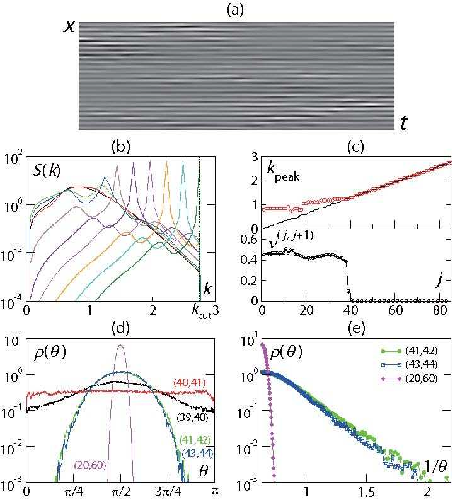
\includegraphics[width=0.45\textwidth]{../figs/YaTaGiChRa08fig2}
 (b)~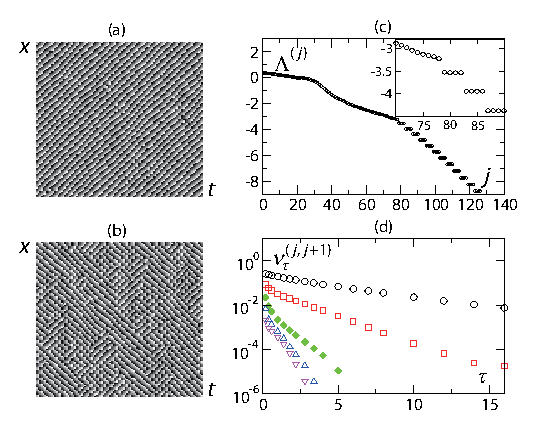
\includegraphics[width=0.45\textwidth]{../figs/YaTaGiChRa08fig3}
\caption{
(left panel)
Fig.~2 of Yang \etal\rf{YaTaGiChRa08}:
Properties of covariant Lyapunov vectors for the KS system
($L = 96$, $k_{\rm cut} = 42 \cdot 2\pi/L$, and PBC).
(a) Spatiotemporal plot of a typical vector in the isolated region
($j=46$, total time $100$).
(b) Spatial power spectra of vectors of indices
$j = 1$, $16$, $32$, $38$, $44$, $52$, $60$, $68$, $76$, $84$
(from left to right in peak position).
(c) Top panel: peak wavenumber in the power spectra (red circles)
and $k = [j/2] \cdot 2\pi/L$ (black line).
Bottom panel: DOS violation fraction $\nu^{(j,j+1)}_\tau$ for pairs of
neighboring vectors (pairs within the same step are omitted).
(d) Angle distributions between pairs of vectors.
(e) Same as (d) but with a different abscissa.
(right panel)
Fig.~3 of Yang \etal\rf{YaTaGiChRa08}:
Complex Ginzburg-Landau equation in the amplitude turbulence regime
($L = 64$, $k_{\rm cut} = 31 \cdot 2\pi/L$, and PBC).
(a,b) Spatiotemporal plots of the phase component of a typical vector $j = 91$ in the isolated region
(same trajectory, but at two distant periods of time, during a total time of $20$ for each plot).
(c) Lyapunov spectrum; inset: close-up around threshold.
(d) Time fraction $\nu^{(j,j+1)}_\tau$ of DOS violation, as a function of $\tau$
($j=78$, 82, 86, 90, 94, from top to bottom).
}
\label{fig:lyapSpecCLG}
\end{figure}



\item[Lyapunov analysis and the collective dynamics of
           large chaotic systems]\rf{TaGiCh09}:
  Not as directly relevant to us as \refref{YaTaGiChRa08}.
  They show, using globally-coupled
  (a) limit-cycle oscillators
  (b) noisy logistic maps,
  that the collective dynamics of large chaotic
  systems is encoded in their Lyapunov spectra: most modes
  are typically localized on a few degrees of freedom, but
  some are delocalized, acting collectively on the
  trajectory. For globally-coupled maps, they show moreover a
  quantitative correspondence between the collective modes
  and some of the so-called Perron-Frobenius dynamics.


\item[An efficient method for recovering Lyapunov vectors] from
singular vectors\rf{WoSa07}: {\bf Predrag 2009-10-15} Wolfe
and Samelson seem to be the most important article to
understand. If Ginelli \etal\rf{ginelli-2007-99} say the key
thing (how to compute covariant eigenvectors, actually) they
hide it well.
Wolfe and Samelson say: `` Standard techniques for computing
Lyapunov vectors produce results which are norm-dependent and
lack invariance under the linearized flow. An efficient,
norm-independent method for constructing the n most rapidly
growing Lyapunov vectors from $n\!-\!1$ leading forward and n
leading backward asymptotic singular vectors is proposed. The
Lyapunov vectors so constructed are invariant under the
linearized flow in the sense that, once computed at one time,
they are defined, in principle, for all time through the
tangent linear propagator. An analogous method allows the
construction of the n most rapidly decaying Lyapunov vectors
from n decaying forward and n-1 decaying backward singular
vectors. ''

\item[From synchronization to Lyapunov exponents and
              back]\rf{PoGiYaMa06}:
The early paper in this series.
In the first part they discuss a general approach to determine
Lyapunov exponents from ensemble- rather than time-averages.
The approach passes through the identification of locally
stable and unstable manifolds (the Lyapunov vectors), thereby
revealing an analogy with generalized synchronization. The
method is then applied to a periodically forced chaotic
oscillator. The
analytical calculations are carried out for a model, the
generalized special flow, that they construct as a simplified
version of the periodically forced R\"ossler oscillator.

\item[Structure of characteristic {L}yapunov vectors in
      spatiotemporal chaos]\rf{PaSzLoRo09}:
They study Lyapunov vectors (LVs) corresponding to
the largest Lyapunov exponents in systems with spatiotemporal
chaos. They focus on characteristic LVs and compare the results
with backward LVs obtained via successive Gram-Schmidt
orthonormalizations. Systems of a very different nature such
as coupled-map lattices and the (continuous-time) Lorenz `96
model exhibit the same features in quantitative and
qualitative terms. They propose a minimal
stochastic model that reproduces the results for chaotic
systems.

\item[The predictability of a flow] which possesses
                many scales of motion\rf{lorenz69},
AKA Lorenz 1969 36-variable method is beloved by weathermen:
we might consider using it as a test of our higher-dimensional 
visualizations.

\item[Periodic orbits, Lyapunov vectors, and singular
    vectors] in the Lorenz system\rf{TrePan98}:
{\bf Predrag 2009-10-15} Trevisan and Pancotti apparently
need to be cited for the observation that covariant vectors
reduce to Floquet eigenvectors in the particular case of a
periodic orbit (seems so obvious it is in ChaosBook without
attribution, and Ruelle and Eckmann\rf{eckerg} surely say
that... Wolfe and Samelson\rf{WoSa07} are inspired by this
article, but seem to go beyond it. Trevisan and Pancotti say
``
A periodic orbit analysis in the Lorenz system
and the study of the properties of the associated tangent
linear equations are performed. A set of vectors are found
that satisfy the Oseledec (1968) theorem and reduce to
Floquet eigenvectors in the particular case of a periodic
orbit. These vectors, called Lyapunov vectors, can be
considered the generalization to aperiodic orbits of the
normal modes of the instability problem and are not
necessarily mutually orthogonal. The relation between
singular vectors and Lyapunov vectors is clarified. The
mechanism responsible for super-Lyapunov growth is shown to
be related to the nonorthogonality of Lyapunov vectors. The
leading Lyapunov vectors, as defined here, as well as the
asymptotic final singular vectors, are tangent to the
attractor, while the leading initial singular vectors, in
general, point away from it. Perturbations that are on the
attractor can be found in the subspace of the leading
Lyapunov vectors.
    ''

\item[On the concept of stationary {L}yapunov basis] by Ershov
and Potapov\rf{ErshPot98}, available on
\HREF{http://www.math.ualberta.ca/~apotapov/Publications.htm}
{http://www.math.ualberta.ca/$\sim$apotapov}. They establish
existence of `stationary {L}yapunov basis'
$\{\jEigvec[1],\cdots,\jEigvec[d]\}$ (called elsewhere `covariant
Lyapunov vectors') such that the Lyapunov
exponents are given by
\beq
    \eigExp[j] = \lim_{N \to \infty} \frac{1}{N}
         \sum_{n=1}^{N} \ln
    |\jEigvecT[j](\ssp_n) \cdot \jMps(\ssp_n) \jEigvec[j](\ssp_n)|
\ee{ErshPotMap}
for a map, and
\beq
    \eigExp[j] = \lim_{T \to \infty} \frac{1}{T}
         \int_0^{T}
    \jEigvecT[j](\ssp_n) \cdot \Mvar(\ssp_n) \jEigvec[j](\ssp_n)
\ee{ErshPotFlow}
for a flow. They say Goldhirsch, Sulem and Orszag\rf{GoSuOr87}
did the same thing, but for ODEs rather than maps. We should also
talk with Dieci\rf{DiEl08,DiRuVl97,DiVl02}
as he is at GaTech and seems to have
worked on closely related problem, the singular value decomposition
(SVD) to approximate Lyapunov spectra.


\item[Computing {L}yapunov spectra] with continuous
         {Gram-Schmidt} orthonormalization.
Christiansen and Rugh\rf{ChRu97},
present a
  continuous method for computing the Lyapunov
  spectrum for a PDE dynamical. They introduce a
  stability parameter and augment system with
  an orthonormal $k$-dimensional frame and a Lyapunov vector such
  that the frame is continuously Gram-Schmidt orthonormalized
  and at most linear growth of the dynamical variables is
  involved. We prove that the method is strongly stable when
  where is the $k$th Lyapunov exponent in descending order and we
  show through examples how the method is implemented.

\item[Improved Numerical Floquet
Multipliers]\rf{Lust01} by
\HREF{https://perswww.kuleuven.be/~u0006235/}
     {Kurt Lust}.  {\bf 2009-09-14 Ruslan}:
Looks like  in this paper {Lust} has proposed a method. If you
could get it for me, it would be great. {\bf 2009-09-14 Predrag
to Ruslan}: You probably do not need to read this paper.
But - for future reference - his
     code for these calculations is
\HREF{https://perswww.kuleuven.be/~u0006235/ACADEMIC/r_psSchur.html}
     {available here}, and
\HREF{https://perswww.kuleuven.be/~u0006235/ACADEMIC/r_PDEcont.html}
     {PDEcont library}  for continuation and bifurcation analysis
      of large scale systems might be of interest.
Their ``A numerical and analytical study of Floquet
        multipliers of periodic solutions near
        a homoclinic orbit''\rf{ZhLuRo01}
might also come in handy.
He used to be a part of the Keller, Doedel, Wulff, Krauskopf,
Hinke crowd.


\item[Are bred vectors the same as
    {L}yapunov vectors?]\rf{KaCoCa02}: {\bf Predrag
2009-10-13} Bred vectors, introduced by Kalay, might have
inspirational value for us, as the atmospheric people
visualize them as spatiotemporal structures. They say:
    ``Bred vectors (BVs) are, by construction, closely
related to Lyapunov vectors (LVs). In fact, after an
infinitely long breeding time, and with the use of
infinitesimal amplitudes, bred vectors are identical to
leading Lyapunov vectors. In practical applications,
however, bred vectors are different from Lyapunov
vectors in two important ways: a) bred vectors are
never globally orthogonalized and are intrinsically
local in space and time, and b) they are finite
amplitude, finite time vectors. These two differences
are very significant in a very large dynamical system.''


\item[Four-dimensional variational assimilation]
	{in the unstable subsp. \\
      (4DVar-AUS) and the optimal subspace dimension}\rf{TrIsTa09}:
	\\
{\bf Predrag
2009-11-21} added this just in case we need to predict pipe turbulence.
Trevisan, D'Isidoro and Talagrand say
``A key a priori information used in 4DVar is the knowledge of the
system's evolution equations. They propose a method for taking full
advantage of the knowledge of the system's dynamical instabilities in
order to improve the quality of the analysis. We present an
algorithm, four-dimensional variational assimilation in the unstable
subspace (4DVar-AUS), that consists in confining in this subspace the
increment of the control variable. The existence of an optimal
subspace dimension for this confinement is hypothesized. Theoretical
arguments in favor of the present approach are supported by numerical
experiments in a simple perfect non-linear model scenario. It is
found that the RMS analysis error is a function of the dimension N of
the subspace where the analysis is confined and is minimum for N
approximately equal to the dimension of the unstable and neutral
manifold. For all assimilation windows, from 1 to 5 days, 4DVar-AUS
performs better than standard 4DVar. In the presence of observational
noise, the 4DVar solution, while being closer to the observations, if
farther away from the truth. The implementation of 4DVar-AUS does not
require the adjoint integration.''


\end{description}

\section{QR decomposition}

\begin{description}
\item[2009-10-10 Sara and Predrag] Understood
    \refref{ginelli-2007-99} (might want to check
    \refref{PoGiYaMa06} as well). Still need to copy
    relevant definitions from ChaosBook.org here.
\end{description}

Consider a $d$-dimensional discrete-time dynamical system. Let
$\ssp_{n}\in \pS \subset \reals^d$ denote the \statesp\ point
at time $t_{n}$ and let $\{{\bf g}_{n}^{(\ell)}\}$, $\ell=1,
\ldots d$, be a set of $d$ orthogonal vectors, ${\bf
g}_{n}^{(\ell)} \cdot {\bf g}_{n}^{(k)} = \delta_{\ell k}$,
that span the tangent space $T\pS$ of the flow at time $t_{n}$.
Collect these into the $n$th \emph{GS basis} (or GS fundamental
matrix), written as the orthogonal matrix
\[
{\bf G}_n = ({\bf g}_n^{(1)} , \ldots ,  {\bf g}_n^{(d)})
\]
whose columns are the basis vectors $\{{\bf g}_{n}^{(\ell)}\}$.
Start now at $t_{n-1}$. Iterating the evolution equations once
maps the ${\bf G}_{n-1}$ orthogonal basis into a set of
non-orthogonal, non-unit basis vectors $\overline{\bf G}_n =
(\overline {\bf g}_n^{(1)} , \ldots , \overline {\bf
g}_n^{(d)})$,
\[
\overline {\bf g}_n^{(\ell)} =\jMps_{n-1}
            \, {\bf g}_{n-1}^{(\ell)}
\,,
\]
where $\jMps_{n-1}$ is the \jacobianM\ of the
transformation evaluated at time $t_{n-1}$.
The $n$th GS basis is now obtained by applying the
Gram-Schmidt orthogonalization to the vectors
$\overline {\bf g}_n^{(\ell)}$. Pick
$\overline{\bf g}_n^{(1)}$ as the direction of the first
Gram-Schmidt vector,
${\bf g}_n^{(1)} = \overline{\bf g}_n^{(1)}/|\overline{\bf g}_n^{(1)}|$.
Pick the component of
$\overline{\bf g}_n^{(2)}$ normal to ${\bf g}_n^{(1)}$
as the direction of the second
Gram-Schmidt vector, normalize to the unit eigenvector,
\bea
{\bf g}_n^{(2)} &=& \frac{1}{|\cdots|}
            \left(\overline{\bf g}_n^{(2)}
                  - (\overline{\bf g}_n^{(2)} \cdot {\bf g}_n^{(1)})
                      \, {\bf g}_n^{(1)}
            \right) \,,
\continue
{\bf g}_n^{(3)} &=& \frac{1}{|\cdots|}
            \left(\overline{\bf g}_n^{(3)}
                  - (\overline{\bf g}_n^{(3)} \cdot {\bf g}_n^{(2)})
                      \, {\bf g}_n^{(2)}
                  - (\overline{\bf g}_n^{(3)} \cdot {\bf g}_n^{(1)})
                      \, {\bf g}_n^{(1)}
            \right) \,,
\nnu
\eea
and so on.
Thus the Gram-Schmidt orthogonalization  amounts to the $\overline{\bf G} =
{\bf Q}{\bf R}$ decomposition, where
\[
\overline{\bf G}_n =
 {\bf G}_n ({\bf G}_n^T \overline{\bf G}_n) =
 {\bf Q}_n {\bf R}_n \,.
\]
The columns of the orthogonal matrix ${\bf Q}_n = {\bf G}_n$
are the elements of the $n$th GS basis, while ${\bf R}_n= {\bf
G}_n^T \overline{\bf G}_n$ is an upper-triangular matrix whose
nonzero elements are obtained by projecting each vector
$\overline {\bf g}_n^{(j)}$ onto the subspace spanned by $\{
{\bf g}_n^{(k)}\}$ with $k \leq j$.
        \PC{${\bf R}_n= {\bf
G}_n^T \overline{\bf G}_n$ formula is reminiscent of the
expression for the \jacobianM\ in terms of fundamental ones,
$\jMps_n= {\bf G}_n {\bf G}_{n-1}^{-1}$.}
        \PC{the reminder of this entry is clippings from \refref{PoGiYaMa06},
        still needs to be edited; there is more QR algebra to fill in. Apologies.
        }

%
%%%%%%%%%%%%%%%%%%%%%%%%%%%%%%%%%%%%%%%%%%%%%%%%%%
\SFIG{GinelliFrames} {}{ \JacobianM\ transports initial
orthogonal frame into a non-orthogonal one. This frame is then
QR decomposed into an $R$-matrix and the next Gram-Schmidt
frame, which is then transported by the next \jacobianM, and so
on. A vector that starts within the subspace spanned by such
finite Gram-Schmidt basis stays within the subspace spanned by
the successive orthogonal frames.
}{fig:GinelliFrames}
%%%%%%%%%%%%%%%%%%%%%%%%%%%%%%%%%%%%%%%%%%%%%%%%%%
%

What we have is a succession of co-moving re-orthogonalized
frames, \reffig{fig:GinelliFrames},
\[
{\bf G}_{n-1} \to \overline{\bf G}_n =
 {\bf G}_n {\bf R}_n
 \to
{\bf G}_{n+1} {\bf R}_{n+1}{\bf R}_n
\]
where ${\bf G}_n$ is an orthogonal frame spanning the tangent
space at $\ssp_n$, and
 \[
{\bf R}_n{\bf R}_{n-1} {\bf R}_{n-1}\cdots {\bf R}_1
 \]
 is the \jacobianM\ computed within the
co-moving frame. It keeps track of stretching along
eigen-directions, but not rotations of the frame, that
information is contained in the imaginary parts of
eigen-exponents of the linearized flow. At each iteration
the linearized flow stretches and squashes the hypercube
whose edges are the $n$th GS basis into a parallelepiped
whose edges are the vectors forming the columns of
$\overline{\bf G}_{n+1}$. Projections of these
vectors onto the $(n\!+\!)$th GS hypercube form
the upper-triangular co-moving frame representation
of the \jacobianM\ $R_{n+1}$.

Ershov and Potapov have shown\rf{ErshPot98} that, by repeating
the above procedure up to a time $t_m$ for $m$ much larger than
$n$,  the GS basis converges to an orthogonal set of vectors
$\{{\bf e}_m^{(k)}\}$, $k=1,\ldots, d$ - the $m$th Gram-Schmidt
vectors - which solely depend on the \statesp\ point
$\ssp_{m}$. Thus the covariant Lyapunov vectors are independent
of where the backward evolution is started along a given
trajectory, provided that it is sufficiently far in the future.
    \PC{For \po s, we need no Ershov and
    Potapov\rf{ErshPot98}. Oseledec arguments are only
    needed for a random long-time ergodic trajectory}

The Lyapunov exponents $\lambda_1 \geq \lambda_2 \geq \ldots
\geq \lambda_d$ are the time-averaged values of the logarithms
of the diagonal elements of ${\bf R}_n$.
        \PC{Ginelli's talk shows that that diagonal elements of ${\bf R}_n$
            are the eigenvalues of the \jacobianM\ $\jMps_n$.}

Assume that a set of Gram-Schmidt vectors at $\ssp_m$ has been
generated by iterating the generic initial condition $\ssp_0$.
Let ${\bf u}_m^{[j]}$ be a generic vector inside the subspace
$\pS^{[j]}$ spanned by $\{{\bf g}_m^{(k)}\}$, $k=1,\ldots, j$,
\ie, by the first $j$ Gram-Schmidt vectors at time $t_m$. This
vector can be iterated backward in time by inverting the
upper-triangular matrix ${\bf R}_m$: if the $c_m^{i}=({\bf
g}_m^{(i)} \cdot {\bf u}_m^{[j]} )$ are the coefficients
expressing ${\bf u}_m^{[j]}$ in terms of the Gram-Schmidt
vectors at $\ssp_m$, then $c_{m-1}^{i}= \sum_k [{\bf
R}_m^{-1}]_{ik} c_m^{k}$. Since ${\bf R}_m$ is
upper-triangular, it is easy to verify that ${\bf u}_n^{[j]}
\in T\pS^{[j]}_n$ at all times $t_n$.


Iterating ${\bf u}_m^{[j]}$ backward for a sufficiently large
number $(m-n)$ of times, it eventually aligns with the
(backward) most expanding direction within $T\pS^{[j]}$. This
defines  ${\bf e}_n^{(j)}$, our intrinsic $j$-th (forward)
expanding direction at the \statesp\ point $\ssp_n$.

In order to verify that ${\bf e}_n^{(j)}$ is covariant, define
the matrix $[{\bf C}_m]_{ij} = c_m^{ij}$,
\[
{\bf C}_m = {\bf R}_m {\bf C}_{m-1}
\,.
\]
By multiplying both sides by ${\bf Q}_m$ and substituting
$\overline {\bf G}_m$ for its QR decomposition on the resulting
right hand side, one is left with ${\bf
e}_{m}^{(j)}=\jMps_{m-1} {\bf e}_{m-1}^{(j)}$ for $j=1,\ldots,
d$.

Covariant Lyapunov vectors $\{{\bf v}_{m}^k\}$ constitute an
intrinsic, covariant basis defining expanding/contracting
directions in \statesp.
In the presence of degeneracies covariant Lyapunov vectors
have to be grouped according to the multiplicity of the
corresponding Lyapunov exponent.

The $i$th Lyapunov exponent is the average of the growth rate
of the $i$th the covariant Lyapunov vector. For 2\dmn\ maps and
3\dmn\ flows this has been shown by B. Eckhardt, D. Yao,
Physica D {\bf 65}, 100 (1993); G. Froyland, K. Judd and A. I.
Mees, Phys. Rev. E {\bf 51}, 2844 (1995); and A. Politi
\etal\rf{PoGiYaMa06}.

Evidence of the validity of the approach was given in
\refref{PoToLe98}, where covariant Lyapunov vectors were
introduced to characterize time periodic orbits in a 1D
lattice of coupled maps. There, it was found that the number
of nodes (changes of sign) in a covariant Lyapunov vectors is
directly connected to the position of the corresponding
Lyapunov exponent within the Lyapunov spectrum.


The covariant Lyapunov vectors are also well defined for
non-invertible dynamics, since it is necessary and sufficient
to follow backward a trajectory previously generated forward in
time. The determination of the covariant Lyapunov vectors is
very efficient. The main computational bottleneck is the memory
required to store the matrices ${\bf R}_n$ and the $n$-time
Gram-Schmidt vectors during the forward integration. The memory
required can be substantially reduced by occasionally storing
the instantaneous configuration in real and tangent space and
re-generating the rest when needed.


\section{2009-09-13 Lyapunov exponents for KS}

% PC 2009-09-12: (b) generated by siminos/figSrc/gnu/lyapSpec.gnu
\begin{figure}
 (a)~\includegraphics[width=0.40\textwidth]{../figs/eigenvalues.ps}
 (b)~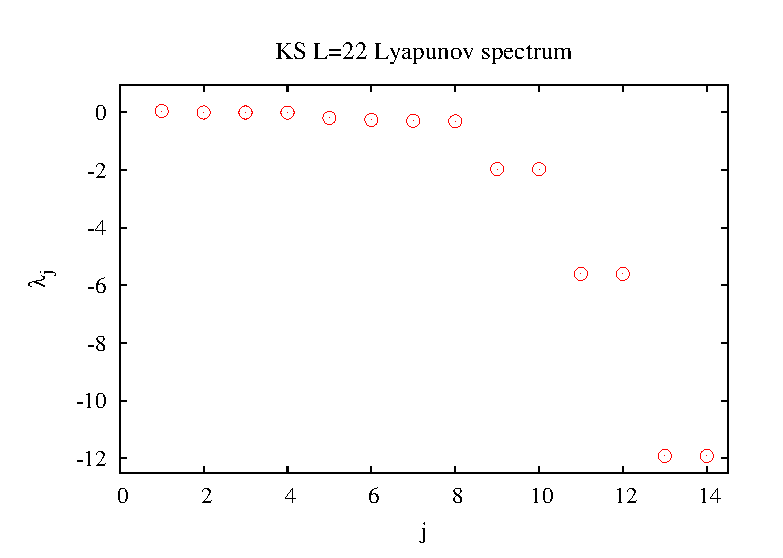
\includegraphics[width=0.50\textwidth]{../figs/lyapSpec}
\caption{
(a)
Lyapunov exponents $\lambda_k$ versus $k$ for the periodic
orbit $\overline{1}$ compared with  the stability eigenvalues
of the $u(x,t)=0$ stationary solution $k^2- \nu k^4$ (from
\refref{Christiansen97}). $\lambda_k$ for $k \geq 8$ fall
below the numerical accuracy of integration and are not
meaningful. Antisymmetric subspace,
hence no \SOn{2}\ pairing of eigenvalues, $N=16$ real Fourier
modes, $L=36.31$. One needs to rescale the time to compare
this to figure (b); -60 in the Lyapunov scale of figure (a)
corresponds to approx. -1.8 in figure (b).
(b)
First 14 Lyapunov exponents $\lambda_j$ for the full
\statesp, periodic b.c. KS for $L=22$, from a 62 real Fourier
modes long-time simulation (from \refref{SCD07}).
}
\label{fig:lyapSpec}
\end{figure}


\begin{description}
\item[Predrag]
Sure looks persuasive, see \reffig{fig:lyapSpec}. I have also
added stability of a periodic orbit from
\refref{Christiansen97}, for KS on the periodic b.c.,
antisymmetric subspace, system size $\tilde{L} = 5.8$ close
to the onset of chaos, 16 real Fourier modes. As (perhaps?)
discussed in \refref{lanCvit07}, one has to be careful about
defining the effective system size $\tilde{L}$ for the
antisymmetric subspace, so these computations are done on
$L=36.31$ (or $L = 18.155$ if one considers the fundamental
$[0,L/2]$ domain only). Going from $(L,\nu) =
(2\pi,0.029924)$ of \refref{Christiansen97} to $(L,\nu) =
(L,1)$ convention used here requires that the time be
rescaled as $t \to \nu t$, and the Lyapunov exponents as
$\lambda_i \to \lambda_i/ \nu = \lambda_i/ 0.029924 $, so -60
in the Lyapunov scale of \reffig{fig:lyapSpec}\,(a)
corresponds to approx. -1.8 on the scale of
\reffig{fig:lyapSpec}\,(b), which would mean that then we
computed only the first pair of isolated eigenvalues. The
reason is that for periodic orbits we are computing {\em
Floquet multipliers} which underflow numerically very
quickly, so we cannot compute many {\em Floquet exponents}.
These covariant Lyapunov eigenvector methods are apparently
much smarter.

In \refref{lanCvit07} computations are done at $L = 38.5$,
but we listed only 4 eigenvalues per periodic orbit, and
considering hopeless organizational skills on the Lan astral
plane, I doubt that the full spectra can be rescued from
Lan's calculations. And, as explained above, probably we cannot
compute them for periodic orbits.

\item[Ruslan]
 Here's the expanded list of Lyapunov exponents for KS with $L = 22$:
 0.048,    0.0,    0.0,   -0.003,   -0.189,   -0.256,   -0.290,   -0.310,
-1.963,   -1.967,   -5.605,   -5.605,  -11.923,  -11.923...
So, there appears to be 8 `physically relevant' exponents and
the rest are pairs of hyperbolically separated ones.

I read
the papers about these covariant Lyapunov vectors and I'm not
sure I understand how they are related to eigenvectors at
periodic orbits: are they aligned?  I suspect that not quite,
apart from the most expanding and the most contracting
direction, the rest are sitting somewhere within the
subspaces spanned by the $k$ most expanding, or $m$ most
contracting eigendirections, but not quite aligned with the
eigendirections themselves.  That's probably why they are
more appropriately called `Lyapunov vectors'.

\item[2009-09-14 Predrag]
The `covariant Lyapunov vectors' are indeed the (right,
non-orthogonal) eigenvectors of the \jacobianM\ \jMps, as
defined in ChaosBook, and coincide with Floquet eigenvectors
for a periodic orbit.

 \item[Ruslan] I use 32 complex Fourier modes, so the
truncated system has 62 degrees of freedom.  The Lyapunov
exponent calculation is standard (using Gram-Schmidt).  The
exponents are the same, independent of the method of
calculation.  I have not attempted to calculate the covariant
Lyapunov vectors. I'm pretty sure that
orthogonality between physical and isolated eigenvectors
applies, but have not checked.

 \item[Ruslan]
It's OK to I email Hong-liu
Yang\rf{YaTaGiChRa08}, ask him to rerun his covariant
Lyapunov vector spectrum for $L=22$, to see whether he agrees
with us.

 \item[Ruslan]
I have the 62 eigenvalues/eigenvectors for all the RPO/PPO
I've detected, but for the highly contracting eigenvalues
the straightforward calculation
suffers from the numerical noise. We need a
better method to compute Floquet multipliers. I have now
checked:   Looks like {Kurt Lust} has proposed one, but I
cannot get his paper on ``Improved Numerical Floquet
Multipliers''\rf{Lust01}. If you could
get it for me, it would be great.

\item[2009-09-13 Ruslan]
``Structure of characteristic Lyapunov
vectors in spatiotemporal chaos''\rf{PaSzLoRo09} states
that characteristic Lyapunov vectors ``reduce to the Floquet
eigenvectors for a periodic orbit'' and references Trevisan
and Pancotti\rf{TrePan98}, which I cannot get electronically.

\item[2009-09-14 Predrag]
I added abstracts of these papers to the reading list above.
The `covariant Lyapunov vectors' are indeed the (right,
non-orthogonal) eigenvectors of the \jacobianM\ \jMps, as
defined in ChaosBook, and coincide with Floquet eigenvectors
for a periodic orbit. For a flow they are defined at a given
\statesp\ point by going back and forward a finite, but
`sufficiently long' time $t$, and coincide with the Floquet
eigenvectors if the point is (relative) periodic. I believed
that for a PDE we cannot go backward, but was wrong; the do
it by using the segment of forward trajectory stored in
memory. The reason why one can get the Floquet {\em exponent}
for arbitrarily long orbit is that the multiplier for eigenvector
evolved in time is just a number, so taking its logarithm over
short time segments and
storing it is trivial, no underflow problems one would get if
one worked with the Floquet {\em multiplier}. So we should be able
to keep track of all 62 eigenvectors, redo it for 126 eigenvectors,
and compare with plots in \refref{YaTaGiChRa08}.
Ginelli \etal\rf{ginelli-2007-99} are the main
reference on the `covariant Lyapunov vectors.' They describe
the QR algorithm for computing Gram-Schmidt vectors (GSV) and
recovering the covariant Lyapunov vectors (CLV) from them.
What confuses me is that so far all papers refer to $\Lyap_j
= \eigRe_j + i \, \eigIm_j$ as purely real, and list only
$\eigRe_j$, but I guess that will be explained somewhere.

\item[2009-09-14 Predrag]
My initial \reffig{fig:lyapSpec} was not optimal; I have now
reploted it as in Fig.~4 of
Yang \etal\rf{YaTaGiChRa08},
agrees with their 'extensivity' plot for $L=96$ and $192$.

I prefer $x$-axis to be $j/\tildeL = 2 \pi j/L$, as in
\reffig{fig:lyapSpecRscld}.

I do not like the way they count eigenvalues:  due to the $\On{2}$
2-dimensional irreducible representations
one should group their $j,j+1$ pairs,
plot them as a single, two-valued $j$, as in
\reffig{fig:lyapSpecRscld}. What one chooses to pair for low
$j$ might be ambiguous, as the nonlinear interactions mix up
the $\On{2}$ 2-dimensional linearly irreducible representations.
Reploted as in our much ignored 1997 paper\rf{Christiansen97},
eigenvalues fall onto $ (2 \pi j/L)^2 - (2 \pi j/L)^4 $
\eqv\ $\EQV{0}$  stability curve.
The isolated `covariant Lyapunov vectors'
are damped by $-(2 \pi j/L)^4$. I worry that we will not have such
amicable divorce for plane Couette and pipe flows...

% PC 2009-09-14: (b) generated by siminos/figSrc/gnu/lyapSpec.gnu
\begin{figure}
 (a)~\includegraphics[width=0.50\textwidth]{../figs/YaTaGiChRa08fig4}
 (b)~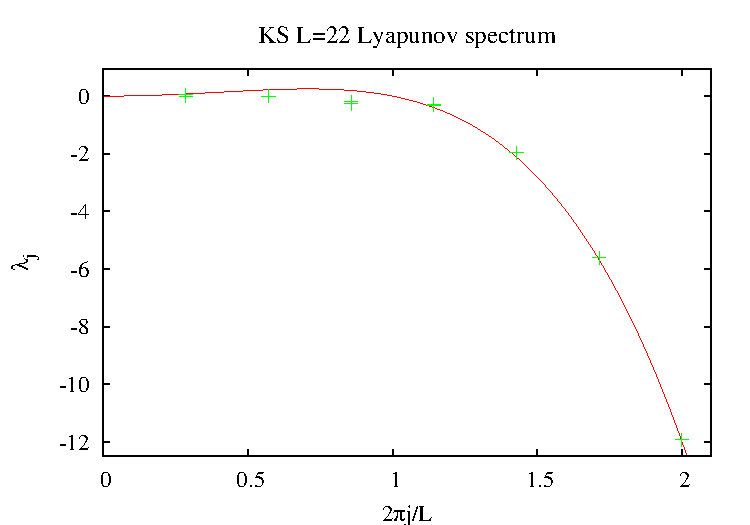
\includegraphics[width=0.40\textwidth]{../figs/lyapSpecRscld}
\caption{
(a)
Fig.~4 of
Yang \etal\rf{YaTaGiChRa08}:
Extensivity of the Lyapunov spectrum for the KS equation with
periodic b.c.. Inset: number of non-negative exponents (circles),
Kaplan-Yorke dimension (squares), metric entropy (diamonds,
multiplied by $50$), and number of physical modes (triangles).
In perfect agreement with
\reffig{fig:lyapSpec}\,(b) here, plotted the same
(incorrect) way.
(b)
First 14 Lyapunov exponents $\lambda_j$ for the full
\statesp, periodic b.c. KS for $L=22$, from a 62 real Fourier
modes long-time simulation (from \refref{SCD07}).
The same as in part (a) and in \reffig{fig:lyapSpec}\,(b), but
abscisa is $j/\tildeL = 2 \pi j/L$, and each $j$ labels
the $\On{2}$ 2-dimensional irreducible representation
Lyapunov exponents pair.  Full line corresponds to
the stability eigenvalues
of the $u(x,t)=0$ stationary solution
$(j/\tildeL)^2- (j/\tildeL)^4$, for arbitrary system size $L$.
}
\label{fig:lyapSpecRscld}
\end{figure}


We also see
that the `physical' modes are split into a less contracting 1/2
and more contracting 1/2 (different slopes in the
\reffig{fig:lyapSpecRscld}\,(a)). We
used to think the first 1/2 is the physically important one,
and say so in the arXiv version 2 of the article.
We stand corrected.

The Floquet eigenvectors of our (relative) periodic orbits are
what they call 'covariant,' so they should fit into their finite back/forth
time vectors like into a glove, whenever the respective state space
points are sufficiently close.

The main point of exploring the ergodic states space hierarchically
by periodic orbits is to tessellate it systematically, in the most
uniform way, by neighborhoods (linearized stable/unstable manifolds)
of periodic points. A periodic solution computed on a small system
size $L$, periodic b.c. is a solution on any multiple of $L$, and it comes
together with a smooth family of corresponding solutions for nearby
$L$'s.

I see prospects of a long and happy marriage here.

\end{description}

\section{2009-09-17  Covariant `transport of vector fields,' a trace formula}

\begin{description}
\item[Predrag] Extracted from \refref{ginelli-2007-99} arXiv source file (might want to check
\refref{PoGiYaMa06} as well):



\item[2009-09-20 Predrag - what's to be done] We presumably have Ruslan's
Floquet multipliers in places like
\\
svn repository vaggelis/production/KS22.0/rpo/ks22rpo016.31\_02.863/Jdiag.dat
\\
(it's hell fishing through the programs, because if there is any description
of what they do and where the data sets are, I have not found them)
but unfortunately they are useless for separating out ``physical'' and
``hyperbolically isolated'' Lyapunov vectors, as they suffer from underflows,
and only a few Floquet multipliers can be computed by methods we have used
so far. We really need to start from scratch and
compute leading 10-20 Floquet {\em exponents}.

Why? If we clear it up for KS,
we have a fighting chance of clearing up the issue for \pCf, where
separating out ``physical'' from
``hyperbolically isolated'' Lyapunov vectors would be a big deal.
Currently Gibson has some 30 eigenvectors for \eqva, but only a handful for
\po s.


\end{description}

\paragraph{
An extract from  ChaosBook.org {appendApplic.tex}, Appendix
{\em Transport of vector fields}
          }
% PC Lyapunov vectors setting up?      	20sep2009
% \section{\EvOper\ for Lyapunov exponents}
% \label{c-vatt-det}
\renewcommand{\ssp}{x}

For higher-dimensional flows only the \jacobianMs\ are
multiplicative, not individual eigenvalues, and the
 evaluation of Lyapunov spectra
requires the extension of evolution equations
to the flow in the tangent space.
The text that follows is clipped from \refref{Vattay}
and the ChaosBook Appendix
\HREF{http://chaosbook.org/chapters/appendApplic.pdf}
     {Transport of vector fields}.
(Probably should also
credit also Lazutkin, I vaguely remember a similar
construction in his work, except that at the moment
I cannot find a reference).
First one determines a periodic orbit, by any scheme.
Once one has it, determine the Lyapunov {\em unit}
vectors by the tangent space eigenvalue
condition, with flow forced by
the (already known) periodic solution. To make it a workable scheme we
need to reformulate this, and instead of computing Floquet
multiplier, evaluate the Floquet exponent along each such
tangent eigen-direction. Shouls be doable, as it is a 1-dimensional
integration. Failing this, we need to learn how other people compute
Lyapunov vectors...

The key idea is to extend the dynamical system by
the tangent space of the flow,
suggested by the standard numerical methods for evaluation of
Lyapunov exponents:      %\rf{BGS80}:
start at $\xInit$ with
an initial infinitesimal tangent space vector in the
$d$-dimensional tangent space
$\eta(0) \in T\pS_{\ssp}$,
and let the flow transport it  along the
trajectory $\ssp(t)= f^t(\xInit)$.

The dynamics in the tangent bundle
$(\ssp,\deltaX) \in  {\bf T}\pS$
is governed by the system of equations of variations:
% \refeq{die}:
%\rf{arnold92}:
	\PC{fix notation: ${\bf(T)}\pS$?}
\[
\dot{\ssp}=\vel(\ssp) \,, \quad
\dot{\eta}=\Mvar(\ssp) \, \eta\, .
%\label{die}
\]
Here $\Mvar(\ssp)$ is % \refeq{DerMatrix},
the {\stabmat} (\velgradmat) of the flow.
We write the solution as
\begin{equation}
x(t)=f^t(\xInit) \,, \quad
 % {\bf \eta}(\xInit,\eta_0,t)
\eta(t)=\jMps^t(\xInit) \, \eta_0 \, ,
\label{xit}
\end{equation}
with the tangent space vector $\eta$ transported by
the {\jacobianM} $\jMps^t(\xInit) = \partial \ssp(t)/ \partial \xInit$.
% \refeq{hOdes}.

% As explained in \refsect{s_lin_stab},
The growth rate of this vector is multiplicative along the trajectory
and can be represented as $\eta(t)=|{\eta}(t)|/|{\eta}(0)| \, u(t)$
where $ u(t)$ is a ``unit" vector in some norm $||.||$.
For asymptotic times and for almost every initial $(\xInit,\eta(0))$,
this factor converges to the leading eigenvalue of the
linearized stability matrix of the flow.

We implement this multiplicative evaluation
of Floquet multipliers by adjoining
the $d$-dimensional transverse tangent space
$\eta \in {\bf T} \pS_x$; $\eta(\ssp) \cdot \vel(\ssp)=0$
to the ($d$+1)-dimensional dynamical evolution
space $x\in \pS \subset \reals^{d+1}$.
	\PC{this looks wrong: $ \vel(\ssp)$ is not normal
            to other eigenvectors. Keep the marginal direction?}
In order to determine the length of the vector $\eta$
we introduce a homogeneous
differentiable scalar function $g(\eta)=||\eta||$.
It has  the property $g(\Lambda \eta)=|\Lambda | \, g(\eta)$
for any $\Lambda $.
An example is the projection of a vector to its $d$th component
\[  %\begin{equation}
 g \left( \begin{array}{c}
	\eta_1 \\
	\eta_2 \\
	\cdots \\
	\eta_d
\end{array} \right)= |\eta_d| \,.
%\label{proj_norm}
\] %\end{equation}

Any vector $\eta(0) \in T\pS_{\ssp}$ can now be represented by the product
$
\eta=\Lambda {u}
$,
where $ {u}$ is a ``unit" vector in the sense that its
norm is $||{u}||=1$, and the factor
\begin{equation}
\Lambda^t(x_0,{u}_0)=g(\eta(t)) = g(\jMps^t(x_0) {u}_0)
\label{lamb_def}
\end{equation}
is the multiplicative ``stretching'' factor.

Unlike the leading eigenvalue of the \jacobianM, the stretching factor is
multiplicative along the trajectory:
\[
\ExpaEig^{t'+t}(x_0,{u}_0)=\ExpaEig^{t'}(x(t),{u}(t))
				\, \ExpaEig^t(x_0,{u}_0).
\]
The ${u}$ evolution constrained to $E {\bf T}_{g,x}$, the space of unit transverse
tangent vectors,
is given by rescaling of (\ref{xit}):
\begin{equation}
%{u}(x_0, {u}_0, t)
{u}'
=R^t(x,{u})=
\frac{1}{\ExpaEig^t(\ssp,{u})} \jMps^t(\ssp) {u} \, .
%{u}(x(t))\in E {\bf T}_{g,x }
\label{R}
\end{equation}

We note  next that if the trajectory $f^t(x)$ is periodic with
period $T$, the tangent space contains $d$ periodic solutions
\[
\jEigvec[i](x(T+t))=\jEigvec[i](x(t)) \,, \quad i=1,...,d ,
\]
corresponding to the $d$ unit eigenvectors $\{\jEigvec[1],
\jEigvec[2], \cdots, \jEigvec[d]\}$ of the transverse stability
matrix, with ``stretching" factors (\ref{lamb_def})  given by
its eigenvalues
\[
\monodromy_p(x) \jEigvec[i](x) = \ExpaEig_{p,i} \, \jEigvec[i](x)
\,, \quad i=1,...,d.
\qquad \mbox{(no summation on $i$)}
\]

\noindent{\bf Predrag} what follows was developed for evaluation
of spectral determinants on the extended, tangent bundle space. Not
sure we need it, but we might... (need stability eigenvalues
to solve Newton equations for eigendirections?)

In order to
compute the stability of the $i$th eigen-direction solution, it
is convenient to expand the variation around the eigenvector
$\jEigvec[i]$ in the stability matrix\ eigenbasis
$
\delta {u} = \sum \delta u_\ell \, \jEigvec[\ell]
\, .
$
The variation of the map (\ref{R}) at a complete period $t=T$
is then given by
\begin{eqnarray}
\delta R^T (\jEigvec[i])  &=&
\frac{\monodromy \delta{u}}{g(\monodromy \jEigvec[i])}
-\frac{\monodromy \jEigvec[i] }{g(\monodromy \jEigvec[i])^2}
\left(
 \frac{\partial g(\jEigvec[i])}{\partial {u}}
	 \monodromy  \delta{u}
\right)
			\nonumber \\
	&=&
\sum_{k \neq i} \frac{\ExpaEig_{p,k} }{ \ExpaEig_{p,i }}
 \left( \jEigvec[k] -\jEigvec[i]
       \frac{\partial g(\jEigvec[i])}{\partial u_k}\right)\delta u_k
\, .
\label{var_R}
\end{eqnarray}
The $\delta u_i$ component does not contribute to this sum
since $g(\jEigvec[i]+du_i\jEigvec[i])=1+du_i$ implies $\partial
g(\jEigvec[i]) / \partial u_i = 1$. Indeed, infinitesimal
variations $\delta{u}$ must satisfy
\[
g({u}+\delta{u})=g({u})=1 \quad \Longrightarrow \quad
\sum_{\ell=1}^d \delta u_\ell
	  \frac{ \partial g({u})}{\partial u_\ell} = 0
\,,
%\label{constra}
\]
so the allowed variations are of form
\beq
\delta {u} = \sum_{k\neq i}
		\left( \jEigvec[k] -\jEigvec[i]
              \frac{\partial g(\jEigvec[i])}{\partial u_k}\right)c_k
    \,, \quad |c_k| \ll 1
\, ,
\ee{eigvNormalz}
and in the neighborhood of the $\jEigvec[i]$ eigenvector
the $\int d{u}$ integral can be expressed as
\[
\int_g d{u} = \int \prod_{k\neq i} dc_k
\, .
\]
%
%The integral over ${u}$ is restricted to
%$ET_{g,x}$, the space of unit tangent vectors
%transverse to the ($d$+1)-dimensional flow,
%is ($d$-1)-dimensional. For example, if the norm is such that
%the Euclidean length of $ {u}$ is 1,
%this space is a ($d$-1)-dimensional unit hemisphere,
%and if the norm is given by (\ref{proj_norm}), $ET_{g,x}$
%is the ($d$-1)-dimensional hyperplane fixed by condition $\eta_d=1$.
Inserting these variations into the $\int d{u}$ integral we obtain
\begin{eqnarray}
\int_g d{u}\, &&
\prpgtr{ \jEigvec[i]+\delta{u} -R^{T}(\jEigvec[i])
				-\delta R^T(\jEigvec[i]) + \dots}
	\nonumber \\
= \, && \int \prod_{k\neq i} dc_k \,
	\prpgtr{(1-\ExpaEig_{k}/\ExpaEig_{i}) c_k + \dots }
	\nonumber \\
	&&= \prod_{k\neq i} \frac{ 1}{ \left| 1-
			{\ExpaEig_{k} / \ExpaEig_{i } }\right|}
\, .
\nonumber
\end{eqnarray}
Ershov and Potapov\rf{ErshPot98} use the more customary
$\jEigvecT[j] \cdot \jEigvec[j] =1$ norm. That replaces
\refeq{eigvNormalz} by a more familiar looking formula
\beq
\delta \jEigvec[j] = \sum_{k\neq j}
		\frac{\jEigvecT[k] \cdot \delta {\bf M} \, \jEigvec[j]}
              {\alpha^{(k)} - \alpha^{(j)}}
       \jEigvec[k]
\, ,
\ee{eigvNormalzEP}
${\bf M} = \jMps^T \jMps$, with eigenvalues $\alpha^{(j)}$,
where everything is evaluated at time $t$. They credit Landau
and Lifshitz
{\em Quantum Mechanics}\rf{Landau59c} for this formula.

\section{2009-10-10  Covariant Lyapunov vectors, an algorithm}

\begin{description}
\item[2009-10-10 Sara and Predrag] Understood
\refref{ginelli-2007-99} (might want to
check \refref{PoGiYaMa06} as well).
\end{description}

\paragraph{
A general method to
determine covariant Lyapunov vectors in both discrete- and
continuous-time dynamical systems.
            }

The Benettin \etal\rf{bene80a} algorithm to calculate the
Lyapunov exponents relies on construction of orthogonal sets of
Gram-Schmidt vectors. They  are not covariant, \ie, the
Gram-Schmidt vectors at a given \statesp\ point are not mapped
by the linearized dynamics into the Gram-Schmidt vectors of the
forward images of this point. In contrast, the \jacobianM\
$\jMps_n$ eigenvectors \jEigvec[i] also span the
$d$-dimensional tangent space, but are generically not normal.
In numerical work, frequent Gram-Schmidt re-orthogonalization
of the tangent coordinate frame is necessitated by the
exponential growth-rate separation along $\jMps_n$
eigendirections as $n$ increases; for a long orbit direct
computation of eigenvalues of $\jMps_n$ yields a set of
exponentially separated leading multipliers
$\{\ExpaEig_1,\ExpaEig_2,\cdots\}$, subset of which can
resolved within a given machine precision.

The method of \refref{ginelli-2007-99} enables computation of
{\em all} eigenvectors of $\jMps_n$. The two key ides are:
\begin{enumerate}
  \item
Due to the upper-triangular structure a Gram-Schmidt
re-orthogonalization matrix ${\bf R}_n$, a vector $\deltaX$
that starts within the tangent subspace $\deltaX \in
T\pS_{\ssp}^{[j]}$ spanned by the first $j$ Gram-Schmidt basis
vectors, {\em stays} within that subspace spanned by a comoving
frame under subsequent evolution and re-orthogonalizations.
\item Once a set of $\{{\bf R}_1,{\bf R}_2,\cdots,{\bf R}_n\}$
along trajectory $\{\ssp_1,\ssp_2,\cdots,\ssp_n\}$ has been
computed and stored in the memory, it can be used to describe
the action of the the linearized flow \jacobianM\ $\jMps_n$
both \emph{forward} and \emph{backward} in time.

So far, this is true of any QR decomposition. Now to
hyperbolic dynamics; order the \jacobianM\ $\jMps_n$
eigenvectors \jEigvec[\ell] by the real parts of their
eigen-exponents, and let $T\pS^{[j]}$ be the tangent
subspace spanned by the leading $j$ eigenvectors.

Strongly contracting $\ExpaEig^{(j)}$ multiplier forward in
time, becomes the leading $1/\ExpaEig^{(j)}$ multiplier
backward in time. Matrix power method then pulls out this
eigenvalue as the leading one within the subspace
$T\pS^{[j]}$. \emph{Presto:} Increase the dimension of the
subspace by one, and you get the next $\ExpaEig^{(j+1)}$.
Repeat, and you get all eigenvalues and eigenvectors, even
those insanely contacting ones, like $\ExpaEig^{(j)}
\approx 10^{-137}$.

\end{enumerate}
\emph{Bonus points:}
\begin{enumerate}
  \item For periodic orbits we need to evaluate ${\bf R}_n$ for
  only one traversal of the cycle: the method then yields {\em
  all} Floquet vectors and Floquet exponents (no need to mess
  with convergence of `Lyapunov' eigenvectors). As unstable \po
  s fill the ergodic component of the \statesp\ hierarchically,
  their linearized stable / unstable manifolds tessellate the
  stable / unstable foliation with exponentially increasing
  accuracy. No need to explore the \statesp\ by mindless
  numerics, starting with a random initial point. \PC{for
  ChaosBook; define Floquet vector to be eigenvector, so change
  all `Floquet eigenvectors' to `Floquet vectors.'}

  \item \emph{Unexpected bonus:} Near-orthogonality of
      these eigenvectors appears to separate the women from
      girls. According to Ginelli
      \etal\rf{ginelli-2007-99}, it gives us apparently a
      sharp criterion to count the number of `physical'
      degrees of freedom for a PDE solved on a compact
      domain.
\end{enumerate}

A coordinate-independent, local decomposition of \statesp\
into covariant Lyapunov directions is called Oseledec
splitting\rf{ruelle79,eckerg}.
Its numerical implementation in \refref{ginelli-2007-99}
is based on forward/backward
iterations of the tangent dynamics and determination
a set of dynamics covariant directions,
called `covariant Lyapunov vectors (CLV).'

\begin{description}
  \item[Ruslan 2009-10-14] I'm sorry to ruin your optimism
      here, but I don't think this procedure is numerically
      stable: The round-off errors will spill outside
      $T\pS^{[j]}$ and then $1/\ExpaEig^{(k)}$ multipliers
      for $k > j$ will stretch these errors.

\item[Predrag 2009-10-15]
You are right that as it stands, we have not explained the
algorithm. The answer seems to be in Wolfe and
Samelson\rf{WoSa07} (above and in ChaosBook.org/library, link
below), perhaps the most important article to understand.
If Ginelli \etal\rf{ginelli-2007-99} say the key thing (how
to compute covariant eigenvectors, actually) they hide it
well.

  \item[Ruslan 2009-10-14]
Another thing that you have noticed is that they don't say
anything about complex eigenvalues.  This is because in the
construction of the algorithm they assume that all Lyapunov
exponents are distinct, which implies that all Floquet
multipliers of periodic orbits are real and distinct as well
(Even though they write $\lambda_1 \geq \lambda_2 \cdots$
instead of $>$, this is mentioned in one of the papers you
discussed above, but I don't remember which one).  I just
hope that, if we do have a pair of complex conjugate
eigenvalues, the corresponding two Lyapunov vectors will span
the same subspace as the real and imaginary parts of the
corresponding eigenvector.  But this needs to be verified.

\item[Predrag 2009-10-15]
You are right that Wolfe and Samelson\rf{WoSa07} cannot prove
that their method converges for degnerate sets of eigenvalues
(complex pairs being a particular case - real parts are
equal, and the method maps orhtogonal frame to orthogonal
frame, codes stretching/shrinking into $R_{ij}$ matrix,
ignores frame rotations. Ginelli \etal\rf{ginelli-2007-99}
deal with complex eigenvalues (see the plots I copied to the
blog above), so I guess it works. I might ask Takeuchi how
they really do it, Chat\'e says he is smart.

  \item[Ruslan 2009-10-14]
 This may be the best
algorithm we have for determining Lyapunov vectors along a
typical chaotic orbit, but if we want to determine them for a
PO or a RPO, then I think that the best way to do this is to
find out how to solve the eigen-problem for a very badly
conditioned matrix $J$ which can be represented as a product
$J = J_{n}J_{n-1}\cdots J_1$ of not-so-badly conditioned
matrices $J_j$.  You seem to have something along these lines
in the extract 'Transport of vector fields' above, but I
would prefer to see this construction done for maps, since
\emph{computers don't do flows}.


\item[Predrag 2009-10-15]
It's usually easier for maps than flows, and as this is all
formulated for finite times, I think it works for discrete
and continuous finite times equally well. Computers do flows
pretty well, that's how we compute \FloquetM\ \monodromy.
Wolfe and Samelson\rf{WoSa07} did not do it for Floquet
eigenvectors. Trevisan and Pancotti (see above, and
\wwwcb{/library} apparently need to be cited for the
observation that covariant vectors reduce to Floquet
eigenvectors in the particular case of a periodic orbit
(seems so obvious it is in ChaosBook without attribution, and
Ruelle and Eckmann\rf{eckerg} surely say that.

\item[Ruslan 2009-10-15]
Sure, all I'm saying is that a flow in a computer is actually
a map, since it's represented by a numerical integration
scheme.  Anyway, I'll read Wolfe and Samelson\rf{WoSa07}
next.  By the way, cannot download Trevisan and Pancotti from
the library, please check the link.  Also, regarding the
relationship between  covariant vectors and Floquet
eigenvectors: I can see that it will work for real distinct
eigenvalues (aka Floquet multipliers), but again it is not
clear how they are related in the case of complex or repeated
eigenvalues.

\end{description}


\section{Separate the women from girls: Hyperbolicity}
\begin{description}
\item[2009-10-10 Predrag]
\end{description}

%
%%%%%%%%%%%%%%%%%%%%%%%%%%%%%%%%%%%%%%%%%%%%%%%%%%
\SFIG{gin99angle}
{}{
(a) Probability distribution of the angle between stable and
unstable manifold for the H\'enon map $x_{n+1} = 1 -1.4\,
x_n^2 + 0.3 x_{n-1}$, and the Lozi map $x_{n+1} = 1
-1.4\,|x_n| + 0.3 x_{n-1}$ (black line, rescaled by a factor
10). (b) Ignore this frame.
}{fig:gin99angle} %{Hyp}
%
%%%%%%%%%%%%%%%%%%%%%%%%%%%%%%%%%%%%%%%%%%%%%%%%%%
%
A dynamical system is said to be \emph{hyperbolic} if its
\statesp\ has no homoclinic tangencies, \ie, the stable and
unstable manifolds are everywhere transversal to each other.
Since covariant Lyapunov vectors correspond to the local
expanding/contracting directions, one can compute their
relative transversality and quantify the degree of hyperbolicity.
The knowledge of the covariant Lyapunov vectors allows testing hyperbolicity by
determining the angle between each pair $(j,k)$ of expanding
($j$) and contracting ($k$) directions
\[
\phi_n^{j,k} = \cos^{-1}(|{\bf v}_n^{(j)} \cdot{\bf v}_n^k|) \in [0,\pi/2]
\,.
\]
As a test, Ginelli \etal\rf{ginelli-2007-99} compute the
probability distribution $P(\phi)$ of $\phi_n^{1,2}$ for the
H\'enon and Lozi two-dimensional maps. Arbitrarily small
angles are found for the H\'enon map, while the distribution
is bounded away from zero in the Lozi map \reffig{fig:gin99angle},
consistent with the common belief that
only the Lozi map is hyperbolic \rf{CoLe84}.

\begin{description}
\item[2009-10-15 Predrag]
Added references \refref{WoSa07,KaCoCa02,TrePan98,PaSzLoRo09}
(discussed above) to
\wwwcb{/library}. As far as I can tell, the important one is
\refref{WoSa07}.

\item[2009-10-15 Predrag to Ruslan]
I have lost interest in quotienting $\SOn{2}$? Nothing could
be further from the actual state of affairs. Ashley Willis
has made a slice work for a down-stream traveling wave in
pipe (downstream we have pure $\SOn{2}$, and for
angular-traveling waves we have $\On{2}$), and we might soon have a
neighborhood spiral-out. His plots of $\dot{\theta}$ already
show hiccups with velocity going large every so often.

But computing Lyapunov vectors seems important as well. I've
put all the papers you did not yet read onto the
\wwwcb{/library}.

\item[2009-10-15 Ruslan]
I believe slices will work for traveling waves and other
types of relative steady (or nearly steady) states, but not
for generic \rpo s and other 'moving' states.  There we will
probably have to learn how to live with a discontinuous
$\theta(t)$.

\item[2009-10-29 Predrag] Tend to agree.

%\RLDedit{
%\item[2009-10-15 Ruslan]
%I cannot download Trevisan and Pancotti from
%the library, please check the link.
%}
%
%\item[2009-10-15 Predrag]
%Sorry, forgot the *.pdf suffix - now Trevisan and Pancotti is
%downloadable from the library.
%
\end{description}

\section{2009-10-27 ``Lyapunov analysis'' workshop}
\label{iscpif}

\begin{description}

\item[2009-10-27 Predrag] Evangelos (physicist formerly known
as Vaggelis) and I are at the ``Lyapunov analysis from theory
to geophysical applications,''
\HREF{http://iscpif.fr/LTG09}{www.iscpif.fr/LTG09} meeting with
all the Lyapunov heavies. I have put the Ginelli, Pikovsky and
Talagrand talks into \wwwcb{/library}; all talks are eventually
meant to be on their website.
\end{description}

\begin{itemize}
  \item F. Ginelli, {\em Characterizing dynamics with
      covariant Lyapunov vectors.} Please read this, it
      addresses directly the questions in the blog above,
      concerning details of the QR algorithm. Francesco
      credits Abarbanel \etal\rf{AbBrKe91,AbBrKe91a} and
      Politi \etal\rf{PoToLe98} for earlier Lyapunov
      vectors. He says that the distinction from the Wolfe
      and Samelson\rf{WoSa07} `intersection algorithm' is
      that their key formula \beq
   D^{(n)}  y^{(n)} = 0 \ee{eq:WoSa07} is unstable as it
  needs inversion of $D^{(n)}$, whereas the dynamical
  algorithm requires only matrix multiplication and is thus
  more reliable.

Harold Posch -always totally reliable- says that his group
has switched from their older Lyapunov spectra codes to
Ginelli \etal\ algorithm, and it works much better.

  \item G. Radons, {\em Lyapunov modes in extended
      dynamical systems.} See Predrag's notes below.
  \item V. Lucarini, {\em Parametric smoothness and
      self-scaling of the statistical properties of a
      minimal climate model} is closely related to
      Siminos thesis, with 5-dimensional \cLe\ as a
      special case, and a 10-dimensional variant of
      Lorenz that has also 2nd Fourier modes, but (do
      not understand why) those can be rotated
      independently, so the symmetry is
      $\SOn{2}\times\SOn{2}$. He keeps the term that
      accounts for heat generation by viscosity, and
      this seems to break the symmetry.
\begin{description}
\item  Evangelos: Talked to Lucarini. The			
symmetry is $\SOn{2}\times\SOn{2}$ since
the model is a truncation of Boussinesq equation
in two spatial dimensions. Lucarini claims that
the viscosity term does not break the symmetry in
Boussinesq equation but does break it in its truncation.
It sounds more like he does not truncate correctly. Without
the viscosity term his truncation behaves like \cLe\ in the
degenerate case of coexisting, symmetry related attractors.
One should be able to also get a version analogous to the generic
situation in \cLe\ with dynamics along the direction of group action.
\item 
	\ESedit{
Evangelos, 2009-12-2: Read part of Lucarini and Saltzman papers. It appears
that Lucarini is wrong, the system cannot have $\SOn{2}\times\SOn{2}$. 
Boundary conditions in both papers are periodic in $x$ direction and free 
in upper and lower boundary (along the $z$ direction), which implies a vanishing
stream function and vorticity, while we also have $\theta=0$ along the vertical
boundaries. Lucarini uses a complex Fourier expansion in both directions therefore
arguing he has $\SOn{2}\times\SOn{2}$ symmetry, but fails to notice he cannot
satisfy boundary conditions. Saltzman (and of course Lorenz) appears to
get the right truncation by fixing certain terms in his Fourier series (but have
not checked the details of his calculation.)
	}
\end{description}
  \item J. Kurchan, {\em Studying unusually regular or
      unusually chaotic trajectories } uses a bunch of
      cloned trajectories, with probability of cloning
      largest for the extremal values of finite-time
      Lyapunov exponent, in order to detect fine,
      structures, such as minuscule elliptic islands
      within a chaotic sea. Seems to work impressively
      well, and mindlessly detect features that
      otherwise would require real thinking.
  \item G. Morriss, {\em Lyapunov modes for hard
      particles systems} is all about Hamiltonian
      dynamics. It has nice formulas for tangent space
      evolution in $N$-hard balls systems, and physical
      interpretation of `hydro-dynamic' modes.
  \item K. A. Takeuchi, {\em Lyapunov analysis captures
      the collective dynamics of large chaotic
      systems.} Kazamusa AKA Kaz is our best hope for
      computing Floquet eigenvectors for our KS \rpo s,
      unless we do it ourselves.

  \item A. Pikovsky, {\em An introduction to Lyapunov
      analysis
        }
  \end{itemize}
The remaining talks were by the weathermen and women. They were
very fascinating, as there is amazing amount of atmospheric and
ocean data available.
  \begin{itemize}
  \item A. Trevisan and O. Talagrand, {\em On the
      existence of an optimal subspace dimension for
        4DVar }
  \item M. Ghil, {\em Data assimilation and predictability
      in climate models} explained Kalman filters in detail
      that might be useful for including into Lippolis
      thesis. While I am at it; we both heard
      Abarbanel\rf{ACFK09} talk about that, it might be a
      better reference.
  \item G. Lapeyre, {\em Nonlinear singular vectors and
      atmospheric predictability }
  \end{itemize}
The next bunch showed very pretty signatures of
Lyapunov-exponent colored 2-dimensional ocean dynamics and
high atmosphere (Antartic ozon hole) dynamics. Legras has
interesting formulas for diffusion enhanced by stretching
of unstable manifold fronts.
  \begin{itemize}
  \item F. d'Ovidio, {\em Lyapunov analysis for ocean
      front detection }
  \item B. Legras, {\em Transport and Mixing}
  \item E. Shuckburgh, {\em Particle dispersion and
      effective diffusivity }
  \item J. B. Sallee, {\em Observed Lagrangian
      dispersion of surface drifters in the Southern
      ocean }
  \item E. Hernandez-Garcia, {\em Stretching structures
      from finite-size Lyapunov exponents: their impact
      across all biological scales.}
 \item J. Verron and O. Titaud, {\em On the
     assimilation of submesoscale observations into
     ocean models }
  \end{itemize}

\begin{description}
\item[2009-10-29 G. Radons talk]  Gunther says ``orthogonal''
(rather than Gram-Schmidt) vectors. This seems more
descriptive, but I am not sure we should adopt this usage, as
the use of Gram-Schmidt sequential orthogonalizations is
crucial in imposing the upper-triangular structure on $R$'s in
the $QR$ decomposition. CVLs he calls "Lyapunov modes". That is
motivated by thinking of these eigenvectors as a generalization
of `normal modes' of mechanical systems.

In his monograph\rf{PG97} Gaspard talks of ``Mather
decomposition'' (rather than Oseledec); recheck Gaspard's
discussion.
\[
J^t = {\bf f}^{(j)T}(t) \Gamma_j {\bf e}^{(j)}(0)
\]
where ${\bf e}^{(j)}(0)$ are the initial CLVs, ${\bf
f}^{(j)T}(t)$ the final CLVs, and $\Gamma$ encodes
``stretching factors.''

Radons \etal\ central result: Lyapunov modes split in (a)
infinitely many ``trivial,'' hyperbolically decaying modes that
are isolated and do not mix and (b) finite number of
``physical,'' entangled modes, in the tangent space of the
attractor, whose number is proportional to the size $L^D$ of
the $D$-dimensional PDE system. Schematically, the ``physical''
ones are pointing along the `entangled,' physical tangent
directions.

In his talk, Radons shows examples of Lyapunov modes evolving
in time with $\ssp(t)$. Physical ones seem localized,
hyperbolic ones seem very Fourier-mode like. Spatial Fourier
spectrum averaged of the time peaks with increase in $k$, peak
at $k$. Physical ones are flat.

Probability density of angles between adjacent physical
eigenvectors computed over long time is flat, not peaked at
$90^o$, see \reffig{fig:lyapSpecCLG} above. In this way the
`physical' tangent space is transported across the whole curved
strange manifold ergodically, and nonhyperbolicity of the
attractor is used as a test that trajectory initiated along a
given direction stays within the attractor. The `trivial,'
hyperbolically decaying eigen-directions that are isolated
exhibit no such small inter-angles anywhere along the ergodic
trajectory.

The very dramatic drop between decaying and entangled modes is
seen in the Domination of Oseledec Splitting (DOS), a figure in
Yang \etal\rf{YaTaGiChRa08} that I did not include in
\reffig{fig:lyapSpecCLG}. The idea is this: there is always a
long finite time $\tau$ Lyapunov exponent time for which
eigenvalues are correctly ordered. For short a time $\tau$
`physical' ones violate the ordering -\ie, nearby finite time
Lyapunov exponent values cross as $\tau$ increases. They plot a
fraction of the time this happens along a long trajectory, for
a $\tau=0.2$, and for $\tau=2$ - both very sharp. Now,
$\tau=0.2$ seems very short on the scale where shortest
periodic solutions are of order $T=20$. Predrag thinks that DOS
might be more important than angles, as separation should also
work for Smale horseshoes repellers embedded in high
dimensions. Chat\'e says the information in angles is equally
good. {\bf A. Pikovsky} is unconvinced about the angles
approach, and thinks one can construct counter-examples where
it would fail.

While it is very impressive for KS, with physical modes sharply
separated into a low-$j$ rectangle, DOS is not a rectangle for
CGL equation, but more of a sausage along the diagonal, and it
might reflect different kinds of turbulence (`phase' turbulence
vs. `amplitude' turbulence). Predrag thinks quotienting the
symmetry might help, see blog entry of 2009-10-30 below.


\end{description}

\section{2009-12-14 Getting fussy}

\begin{description}
\item[Strict and fussy modes splitting in the tangent space] 
of the Ginzburg-Landau equation
by Pavel V. Kuptsov, Ulrich Parlitz (G\"{o}ttingen University), \HREF{http://arxiv.org/abs/0912.2261v1}{0912.2261v1}. They say:
``
In the tangent space of some spatially extended dissipative
systems one can observe ``physical'' modes which are highly
involved in the dynamics and are decoupled from the remaining set
of hyperbolically ``isolated'' degrees of freedom representing
strongly decaying perturbations. This modes splitting is studied
for the Ginzburg--Landau equation at different strength of the
spatial coupling. We observe that isolated modes coincide with
eigenmodes of the homogeneous steady state of the system; that
there is a local basis where the number of non-zero components of
the state vector coincides with the number of ``physical'' modes;
that in a system with finite number of degrees of freedom the
strict modes splitting disappears at finite value of coupling;
that above this value a fussy modes splitting is observed.
''

The big mystery is that I have met them and wrote ton of notes into
this blog (I believe) but have never found these notes again. Well...
Briefly: I'm impressed with Pavel's computations of covariant vectors.
In his way of computing their relative angles one sees: (1) the separation 
of positive exponents from negative ones (that's what periodic orbit theory likes)
(2) a range of vectors up to Kaplan-Yorke (3) a different range of vectors
up to Ginelli \etal\ cliff.

\end{description}



\renewcommand{\ssp}{a}
